% !TEX root = ../main.tex
\documentclass[../main.tex]{subfiles}

\begin{document}
\section{Development Environment}

\subsection{Sandbox}

\begin{figure}[H]
  \centering
  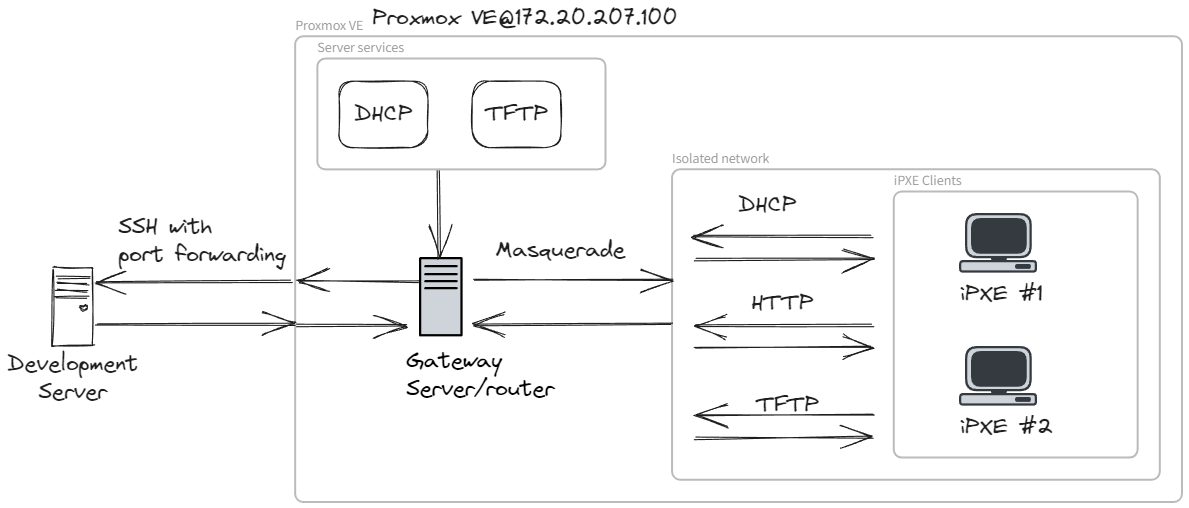
\includegraphics[width=\textwidth]{dev-setup.png}
  \caption{Development Environment}
  \label{fig:dev-setup}
\end{figure}

In order to develop the application without affecting local network a sandbox environment was created using \texttt{Proxmox} \cite{proxmox} virtualization platform.
In total 3 virtual machines were created:

\begin{itemize}
  \item \textbf{Gateway} - A \texttt{Debian} \cite{debian} virtual machine that acts as a gateway between the local network and the sandbox. It is also used as a DNS and DHCP server for the local network
  \item \textbf{iPXE Client \#1} - Virtual machine that is used to test the iPXE booting process. It is also used to test the DHCP and DNS configuration of the gateway
  \item \textbf{iPXE Client \#2} - Virtual machine without an operating system that is used to test the iPXE booting process
\end{itemize}

The only virtual machine that is connected to the local network is the gateway. The other two virtual machines are connected to a private network that is only accessible from the gateway.

\subsection{Gateway services}

The gateway virtual machine is running the following services:

\begin{itemize}
  \item \textbf{SSH Server} - Used to connect to the gateway from development machine. It is also used for port forwarding services running on development machine to the gateway server
  \item \textbf{DNS Server} - Name server for the local network. Accessible only from isolated network
  \item \textbf{DHCP Server} - Used in the IPXE booting process. Accessible only from isolated network
  \item \textbf{TFTP Server} - Provides iPXE boot files. Accessible only from isolated network
\end{itemize}

The DNS, DHCP and TFTP servers are provided by \texttt{dnsmasq} \cite{dnsmasq} service.

\subsection{Gateway configuration}

\subsubsection{SSH Server}

To expose application to the isolated network a remote port forwarding was used. This allows to forward traffic that is coming to the gateway on a specific port to the development machine which
is running the application. This is done by running the following command on the development machine:

\begin{listing}[H]
  \begin{bashcode}
    ssh -NT -R 0.0.0.0:8000:127.0.0.1:8000 hydra-gw
  \end{bashcode}
  \caption{SSH Remote Port Forwarding}
  \label{lst:ssh-remote-port-forwarding}
\end{listing}

This command forwards incoming gateway traffic designated for port 8000 from any IP address (0.0.0.0) to the development machine on port 8000 on the loopback interface.
The \texttt{hydra-gw} is the hostname of the gateway virtual machine. Additionally by providing the \texttt{-NT} flags the command will not open a shell on the gateway machine.

The default ssh server configuration does not allow remote port forwarding to bind to other interfaces than the loopback interfaces.
To allow this functionality the \texttt{GatewayPorts} option in the \texttt{/etc/ssh/sshd\_config} file was set to \texttt{yes}.

\subsection{Routing and NAT}

The gateway virtual machine has two network interfaces:

\begin{itemize}
  \item \textbf{ens18} - Connected to the local network
  \item \textbf{ens19} - Connected to the isolated network
\end{itemize}

To properly route traffic between the two networks the \texttt{net.ipv4.ip\_forward} option in the \texttt{/etc/sysctl.conf} file was set to \texttt{1}.
This option enables IP forwarding in the kernel.
To configure the interfaces the \texttt{/etc/network/interfaces} file was used. The configuration is shown in listing \ref{lst:interfaces-setup}.

\begin{listing}[H]
  \textfile{implementation/code/interfaces-setup.txt}
  \caption{Interfaces setup}
  \label{lst:interfaces-setup}
\end{listing}

The \texttt{ens18} interface is configured to use DHCP to obtain an IP address from the local network. The \texttt{ens19} interface is configured to use a static IP address of \texttt{10.0.0.1}.
Additionally two network bridges were created named \texttt{brout} and \texttt{br0} to represent the local and isolated networks respectively.

To set up dynamic NAT the following \texttt{iptables} rules were added using command:

\begin{listing}[H]
  \textfile{implementation/code/iptables-setup.sh}
  \caption{NAT setup using iptables}
\end{listing}

As by default \texttt{iptables} settings are ephemeral the \texttt{iptables-persistent} package was installed to save the rules to \texttt{/etc/iptables/rules.v4} file.

\subsection{DNS, DHCP, TFTP servers}

\texttt{Dnsmasq} service was used to provide DNS, DHCP and TFTP servers. The configuration is shown in listing \ref{lst:dnsmasq-setup}.

\begin{listing}[H]
  \textfile{implementation/code/dnsmasq.conf}
  \caption{Dnsmasq setup}
  \label{lst:dnsmasq-setup}
\end{listing}

Dnsmasq allows to provide a custom PXE boot file depending on the client architecture (x86 or x86\_64) and target firmware (BIOS or UEFI).
This is done by first defining the vendor class identifiers for each architecture and firmware combination and then providing a custom boot file for each combination.
As the iPXE clients are x86\_64 machines running UEFI firmware only the \texttt{UEFI x86\_64} vendor class identifier was defined.

The DHCP and DNS servers were configured to listen only on the internal and loopback interface addresses. This is done to prevent the services from being exposed to the local network.
Additionally the DHCP option \textbf{6} and \textbf{3} were set to provide clients the information about the DNS server and gateway IP address respectively.
Dnsmasq replaces the (0.0.0.0) IP adress with the host IP address in the DHCP response.



\end{document}